\section{Temperature Encoding Experiments} \label{sec:empirical-studies-temperature-encoding-experiments}

So far we were able to show that symbols improve the effectiveness of the learning process when training neural networks on limited datasets. We have however failed to show that they can generalize to digit combinations that they have not seen before. In Section \ref{sec:theory-approach-methodology-temperature-encoding} we described an alternative representation for our symbols, namely the temperature encoded symbols. We explained our expectation that temperature encodings will improve the ability of the networks to generalize to unseen combinations since they are able to encapsulate three characteristics that are important in developing an algorithm that performs arithmetic. Specifically, these characteristics are, (1) the ability of the symbols to represent the ordinal relationship between digits, (2) the ability to represent the quantity of the digits and (3) the ability to capture the function of the operator. The prior experiment showed that one-hot vectors are capable of capturing the function of the operator, as shown by the ability of the models to internally represent the carry forward behavior of addition. They however fail in providing the other two properties. This final set of experiments investigates the ability of temperature encoded symbols to capture all three characteristics and presents a solution to our problem. 

\subsection{Experiment 6: Temperature Encoding} \label{sec:experiment-6}

\subsubsection{Objective}

When a symbol is represented as a temperature encoded vector, the symbol is represented as an array where a number of consecutive elements equal to the value of the digit being represented are set to one, the rest are set to zero. Figure \ref{fig:temperature-encoding} shows a depiction of a temperature encoded symbol of the number 5. We believe that symbols encoded using this representation can capture the quantitative and ordinal meaning of the digits and would therefore help the recurrent neural network learn an algorithm for arithmetic operations as opposed to simply learning a classifier or mapping function.

The goal of this experiment is to determine empirically whether or not models trained using the temperature encoded symbols have the ability to discover a decision function that can represent the algorithm that performs addition. We constrain the experiment to only use symbols as in Experiment 5. The models accept a sequence of operands encoded in the temperature encoding and outputs values encoded in the temperature encoding as well. The performance of the trained model is tested against both the training set as well as an unseen test set to determine if the model can generalize to unseen combinations of operands. 

\subsubsection{Method}

\begin{figure}
	\centering
	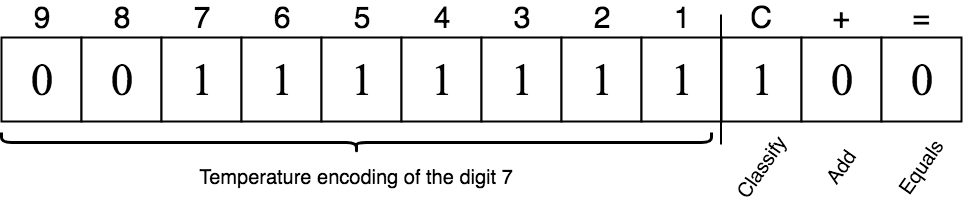
\includegraphics[max width=\textwidth]{experiment-6-input}
	\caption{An example of an input vector for the digit 7 on the first time step. The first nine features are for the temperature encoded symbol. The 10th (C) feature when set, instructs the RNN to output the class at that time step. The 11th (+) feature when set, instructs the network to output the least significant digit of the result. The 12th (=) feature when set, instructs the RNN to output the most significant digit of the result.}
	\label{fig:experiment-6-input}
\end{figure}

Three models are developed that learn to perform addition on temperature encoded symbols. Figure \ref{fig:sequential-model-temperature-symbols} shows an example of a recurrent neural network using temperature encoding to learn to do addition. The models accept a sequence of four vectors 12 elements each. Figure \ref{fig:experiment-6-input} depicts an example input. The first nine elements hold an operand represented as a symbol encoded using a temperature encoding. The 10th element indicates to the network to classify the input, meaning that if it is set to one, the model should output the same input digit using the same temperature encoding. The 11th element indicates the addition operator and the model should output the least significant digit of the result of the addition. Finally, the 12th element represents the equals sign, indicating to the model to output the most significant digit of the result. The output of each of the networks is a nine-element vector that represents the temperature encoding of the output. The following are the various architectures that were tried:
\begin{itemize}
	\item \textbf{Model A}: Two hidden layers, 20 units each.
	\item \textbf{Model B}: Two hidden layers, 10 units each.
	\item \textbf{Model C}: Two hidden layers, 5 units each.
\end{itemize}

\begin{figure}
	\centering
	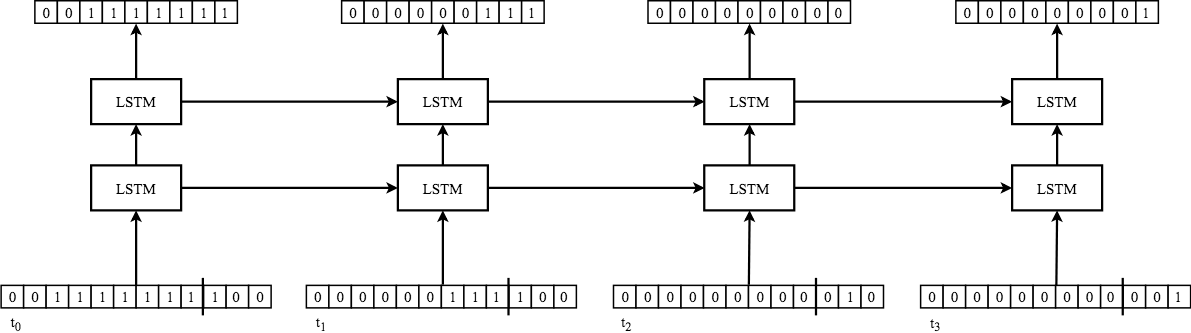
\includegraphics[max width=\textwidth]{sequential-model-temperature-symbols}
	\caption{A sequential model constrained to use symbols only. However, the symbols are encoded using temperature encoding. In this case the model is learning to perform 7 + 3. The output on the third time step (least significant time step) is all zeros to encode 0.}
	\label{fig:sequential-model-temperature-symbols}
\end{figure}

A similar dataset like the one used in Experiment 5 is used for this experiment. A subset of 80 combinations are selected for training from the 100 combinations of operands, making sure that each unique digit would be present at least once on either side of the addition operator. That same training set is also used for validation and as the test set of seen combinations. The remaining 20 combinations are used as the unseen combinations test set. Each model is trained and tested five times and the mean accuracy of each model is recorded when applying both the seen test set and the unseen test set on the trained model. Training is performed over 5000 epochs in batches of 10 using the Adam optimizer algorithm and the mean square error loss function with a learning rate of 0.001. 

\subsubsection{Results}

\begin{table}
	\center
	\caption{A comparison of the mean accuracy of each of the models trained using the temperature encoding when tested on the test set of \textbf{seen} combinations as well as the test set of \textbf{unseen} combinations.}
	\label{tab:experiment-7-results-table}
	\begin{tabular}{ |c|c|c| } 
		\hline
		Model & Accuracy - Seen (\%) & Accuracy - Unseen (\%)\\ 
		Model A & 100.0 & 90.0\\  
		Model B & 100.0 & 93.0\\  
		Model C & 100.0 & 86.0\\  
		\hline
	\end{tabular}
\end{table}

Table \ref{tab:experiment-7-results-table} shows the results obtained for each of the architectures trained. The table presents the mean accuracies of each architecture when tested on both the dataset of seen combinations and the dataset of unseen combinations. 

\subsubsection{Discussion}

\begin{figure}
	\centering
	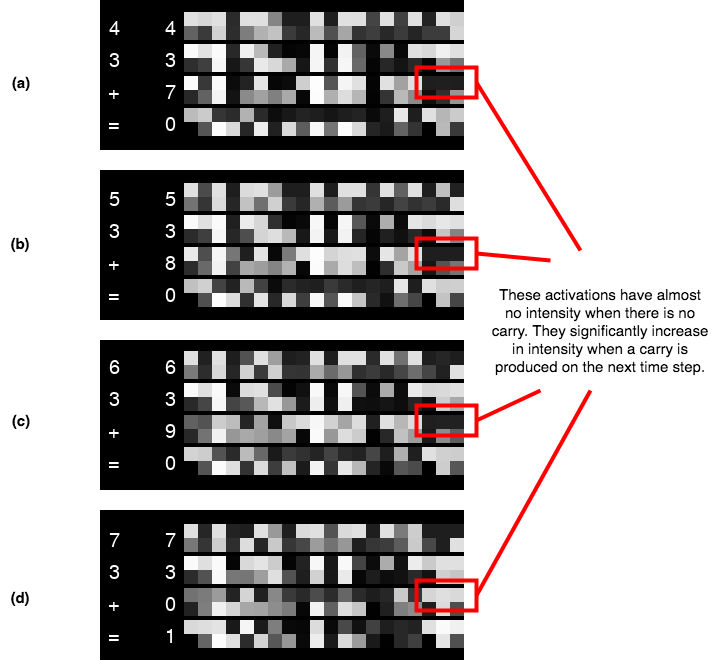
\includegraphics[max width=\textwidth]{activations-cluster-carry-temperature}
	\caption{A series of activations produced when applying examples from the unseen test set to Model A, trained using temperature encoded symbols. The activations show how the intensity in the top right region of the third time step indicates if a carry should be generated.}%
	\label{fig:activations-cluster-carry-temperature}%
\end{figure}

We can see from the results in Table \ref{tab:experiment-7-results-table} that the models perform perfectly on the training combinations and are also relatively successful at generalizing to the unseen combinations. This shows that the temperature encoded symbols that take into account the ordinal nature of the digits allow the recurrent neural networks to capture an algorithm that performs addition.

\begin{figure}%
	\centering
	\subfloat[Activations for 4 + 3]{{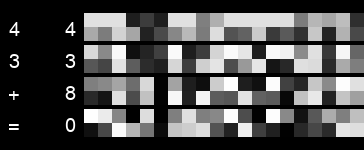
\includegraphics[width=0.5\textwidth]{activations-cluster-no-carry-4-3} }}%
	\subfloat[Activations for 5 + 3]{{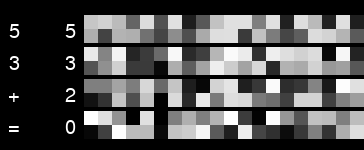
\includegraphics[width=0.5\textwidth]{activations-cluster-no-carry-5-3} }}%
	
	\subfloat[Activations for 6 + 3]{{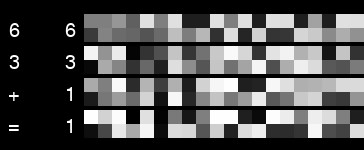
\includegraphics[width=0.5\textwidth]{activations-cluster-no-carry-6-3} }}%
	\subfloat[Activations for 7 + 3]{{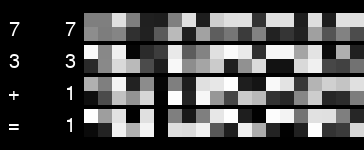
\includegraphics[width=0.5\textwidth]{activations-cluster-no-carry-7-3} }}%
	\caption{A series of activations produced when applying examples from the unseen test set to Model D of Experiment 5, trained using one-hot vector symbols. No discernible patterns are visible.}%
	\label{fig:activations-cluster-no-carry}%
\end{figure}

To further verify this conclusion, we generated activations clusters for a series of combinations from the unseen test set using Model A. Figure \ref{fig:activations-cluster-carry-temperature} shows the activations produced. In addition, Model D from the previous experiment (Experiment 5 in Section \ref{sec:experiment-5}) was retrained making sure that the same combinations shown in Figure \ref{fig:activations-cluster-carry-temperature} are part of the unseen test set. The activations for that model are shown in Figure \ref{fig:activations-cluster-no-carry}. The activations generated by the model trained using the temperature encoded symbols exhibit consistency among the same operands. Also, the region indicated at the top right end of the third time step shows a clearer carry forward signal than the one seen in Figure \ref{fig:activations-cluster-carry-temperature}. When we contrast these activations with the ones shown in Figure \ref{fig:activations-cluster-no-carry} we see that the model trained with one-hot vector symbols do not depict these clear patterns when applied to the unseen test set.

Experiments 5 and 6 show that symbols improve the accuracy of neural networks by aiding the learning algorithm in discovering a representation that capture some aspects of the algorithm that performs the operation. Temperature encoded symbols allow the models to capture more aspects. Specifically, the quantity and ordinal relationship of the operands. This results in better generalization. In the next and final experiment, we replicate Experiment 4 but this time, instead of using the one-hot vectors we use temperature encoded symbols.

\subsection{Experiment 7: Noisy Handwritten Digits with Temperature Encoded Symbols} \label{sec:experiment-7}

\subsubsection{Objective}

In Section \ref{sec:theory-approach-methodology-temperature-encoding} we explained our observation of how humans learn to perform arithmetic. We explained how children in particular learn to represent digits by mapping between the image of a digit and the image of familiar objects. These familiar objects (like apples for example) behave as symbols that convey both quantity and ordinal relationships. The human learner can then act on these symbols to produce a more accurate result. This process allows the human learner to generalize the solution to combinations of digits that they have not experienced before.

We believe a neural network model can be constructed that learns in a similar way. The network is provided a sequence of handwritten digits and an operator symbol. It is trained to develop an internal representation that can map between the image of the digit and a symbol that captures both the quantity and ordinal relationships represented by the digit (the temperature encoded symbol). The model is also trained to perform the arithmetic operation on the two digits. With deep recurrent neural networks, these two related tasks can be combined into one model that can learn to perform both with high accuracy.

The purpose of this experiment is to show that it is indeed possible to build such a model and that the use of symbols represented as temperature encodings can improve the accuracy of training on a restricted dataset as well as force the learning algorithm to discover a representation that can generalize to unseen combinations of digits. We also investigate how varying the amount of symbols present affects the accuracy of the model on the unseen test data.

\subsubsection{Method}

Five recurrent neural network models are developed for this experiment each having the same architecture. Figure \ref{fig:sequential-model-noisy-temperature} shows a diagram of the architecture used. The models accept a sequence of four 28x28 images. The first two images are of the MNIST handwritten digit operands, the third image is the operator (plus, minus, times and divide) consistently rendered in a standard font, and finally the fourth image is an equals sign. The model is trained so that when it sees the operands on each of the first two time steps, it outputs a temperature encoded symbol that represents the digit in the image. When the model is presented with the operator on the input, it performs the operation on the operands and then outputs a temperature encoded symbol that represents the least significant digit of the result. Finally, when the equals sign is presented, the model outputs a temperature encoded symbol representing the most significant digit of the result.

The neural network architecture used is composed of an input layer of 784 units for the 28x28 pixel images. Two hidden layers are used each consisting of 512 LSTM units. The output layer is a vector of nine elements to represent the temperature encoded results. The networks are trained using the Adam optimizer with the mean square error as the loss function and a learning rate of 0.001. Training is performed over 200 epochs in batches of 100 and the model performing best on the validation set is saved.

\begin{figure}
	\centering
	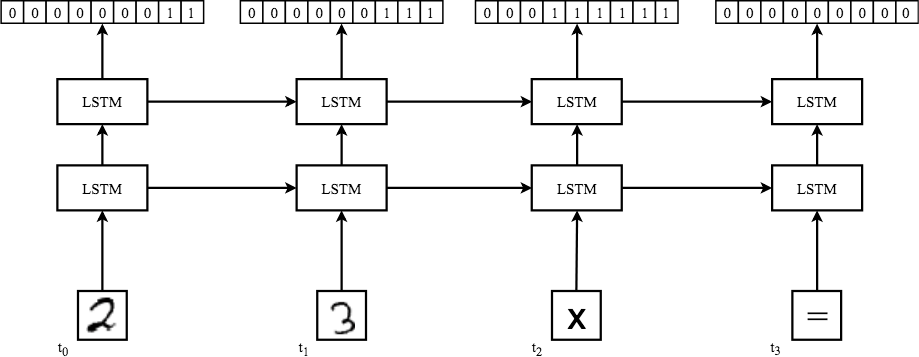
\includegraphics[max width=\textwidth]{sequential-model-noisy-temperature}
	\caption{A sequential model learning to perform arithmetic on images of handwritten digits in the presence of symbols. The symbols are provided on the outputs of the first two intermediate steps using temperature encoding. Here the model is performing multiplication on the combination: 2 x 3.}
	\label{fig:sequential-model-noisy-temperature}
\end{figure}

The same dataset used in Experiment 4 in Section \ref{sec:experiment-4} is also used for this experiment with the exception of replacing one-hot vector symbols with temperature encoded symbols. To recap, for each operator, the combinations of digits are split into a set of seen combinations that includes, 80\% of the combinations of digits. For each of the seen combinations, eight MNIST samples are selected. Four of these samples are used for training, two for validation and the remaining two for testing. The remaining 20\% of the combinations are reserved as the set of unseen combinations that are used to verify that the models have learned an algorithm of the operations. The dataset of seen combinations is replicated five times, each replica includes a different percentage of symbols present. The symbol spreads used are 0\%, 25\%, 50\%, 75\% and 100\%. The symbols were presented as output labels to the first two time steps. The model is trained to classify the handwritten digit with the aid of the symbol provided. When symbols are not provided, a vector composed of 0.5 dummy values is used instead. Each model is trained five times using 5-fold cross-validation.

\subsubsection{Results}

\begin{table}[p]
	\center
	\caption{A comparison of the mean accuracy and standard deviation along with the p-value of a hypothesis t-Test when compared to the 0\% symbols model when tested on the test set of \textbf{seen} combinations.}
	\label{tab:experiment-8-results-table-seen}
	\begin{tabular}{ |c|c|c|c| } 
		\hline
		\% Symbols Present & Accuracy (\%) & Standard Deviation  & p-value\\ 
		0\% & 41.55 & 0.0302 & NA \\  
		25\% & 51.30 & 0.0457 & 0.02311\\  
		50\% & 60.65 & 0.0379 & 0.00049 \\  
		75\% & 75.84 & 0.0587 & 0.00063\\  
		100\% & 84.26 & 0.0582 & 0.00018\\  
		\hline
	\end{tabular}
\end{table}

\begin{table}[p]
	\center
	\caption{A comparison of the mean accuracy and standard deviation along with the p-value of a hypothesis t-Test when compared to the 0\% symbols model when tested on the test set of \textbf{unseen} combinations.}
	\label{tab:experiment-8-results-table-unseen}
	\begin{tabular}{ |c|c|c|c| } 
		\hline
		\% Symbols Present & Accuracy (\%) & Standard Deviation  & p-value\\ 
		0\% & 4.62 & 0.0133 & NA \\  
		25\% & 25.53 & 0.0900 & 0.16889\\  
		50\% & 45.90 & 0.0319 & 0.00199 \\  
		75\% & 54.63 & 0.0324 & 0.0\\  
		100\% & 69.58 & 0.0694 & 0.00088\\  
		\hline
	\end{tabular}
\end{table}

\begin{figure}[p]
	\centering
	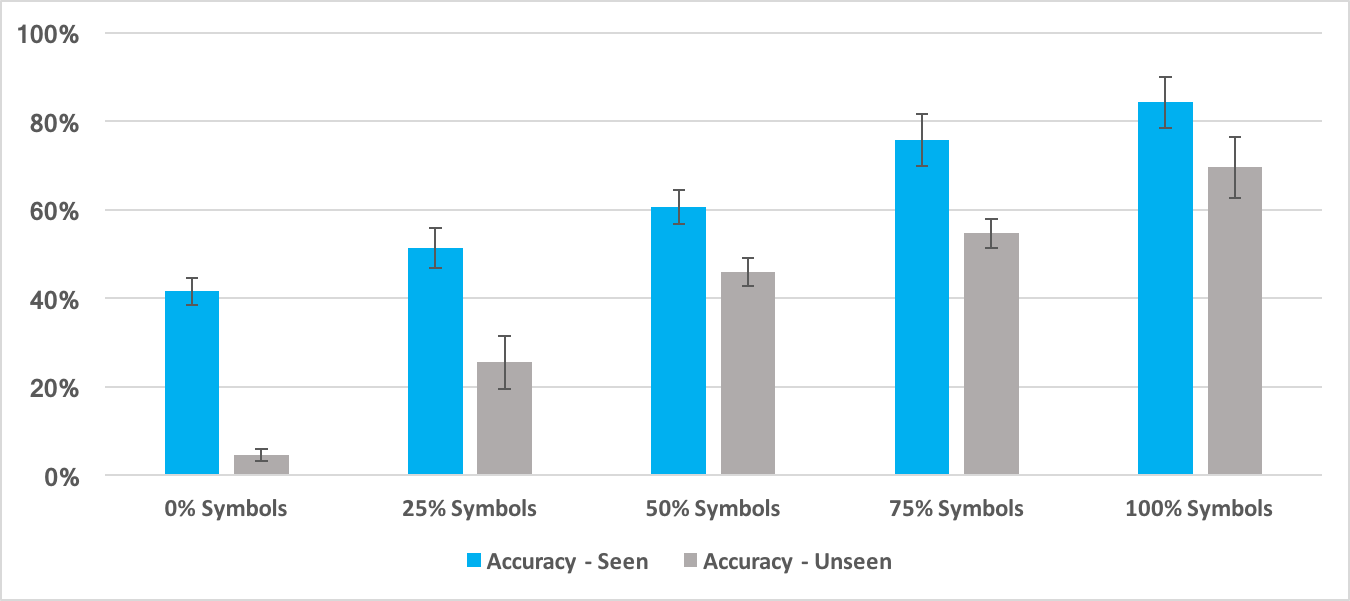
\includegraphics[max width=\textwidth]{experiment-8-results-chart-2}
	\caption{A comparison of the mean accuracy and 95\% confidence intervals for each of the models trained with 0\% to 100\% temperature encoded symbol presence when tested on both the test set of \textbf{seen} and \textbf{unseen} combinations.}
	\label{fig:experiment-8-results-chart}
\end{figure}

Table \ref{tab:experiment-8-results-table-seen} shows the results of testing the models on the test set of seen combinations. Similarly, Table \ref{tab:experiment-8-results-table-unseen} shows the results of testing the model on the test set of unseen combinations. The tables present the mean accuracy, standard deviation and the p-test score for each of the models developed. Figure \ref{fig:experiment-8-results-chart} depicts the mean accuracies along with the 95\% confidence intervals for all five models trained on both the seen and unseen test sets.

\subsubsection{Discussion}

The results show that increasing the number of symbols available per combination during training, improves the accuracy of the recurrent network when tested on combinations the model has seen during training. This result is comparable to Experiment 4 where we had a similar architecture and approach. However, we used a different representation for the symbols, namely temperature encoded vectors. More importantly the results show the accuracy on unseen combinations increases as more symbols are used during training. These results confirm the findings we've observed in several of our previous experiments and also supports our hypothesis that artificial neural networks similar to human learners can benefit from the presence of clear and concise symbols when training using limited datasets.

The results in this experiment show that the way the symbols are represented can have significant effect on the learning ability of the models. The one-hot vector representation was effective for learning a simple mapping function when all combinations of inputs were provided during training. However, it failed to capture the ordinal nature of the digits and therefore they were not able to discover a representation for an algorithm that can perform the arithmetic operations. By using temperature encoded symbols for the digits, the models are able to represent the arithmetic algorithm and generalize to unseen combinations of digits.